\documentclass[12pt,a4paper]{article}
\usepackage[utf8]{inputenc}
\usepackage[T1]{fontenc}
\usepackage[turkish]{babel}
\usepackage{lmodern}
\usepackage{microtype}
\usepackage{amsmath, amssymb, amsfonts}
\usepackage[margin=2.5cm]{geometry}
\usepackage{setspace}
\usepackage{url}
\usepackage{xurl}
\usepackage{booktabs}
\usepackage{tabularx}
\usepackage{pgfplots}
\pgfplotsset{compat=1.18}
\usetikzlibrary{babel}

\onehalfspacing

\title{\textbf{Duran Sicimler Teoremi VII: CERN ALPHA Antimadde Tuzaklarında Öz-Tutarlı Girdap Doyumu, İlk-İlkelerden Hiperince Rezonans Çizgi Şekli ve 511 keV Ore--Powell Spektrum Çözümü} \\[0.3cm]
\large (SDR-EVC Sıfır-Parametreli Eşleşme ve $e^+$ Çapraz Doğrulaması, $1.03/1.07\text{ T}$ Akı Sürüklenmesi ve Analitik $g_{\mathrm{vortex}}$ Çizgi Şekli, Tam 1949 Ore--Powell Düzeltmesi ve BASE-STEP 2026 Karayolu Taşıması Lyapunov Kararlılığı)}
\author{Fahri Meral}
\date{17 Ekim 2026}

\begin{document}
\shorthandoff{=}

\maketitle

\begin{abstract}
Teorem I--VI serisinin devamı olarak bu 7.\ çalışmada, Eylül 2026 Navier--Stokes--FENE-P iç-çekirdek girdap dinamiğinin 2025--2026 CERN antimadde deneylerindeki dört açık laboratuvar/gözlem problemine uygulaması sunulmaktadır:
\begin{enumerate}
    \item ALPHA 2025 SDR-EVC ``dönen duvar'' tork uyuşmazlığı: kaymasız ideal yarıçap $r_p^{\mathrm{ideal}} = 0.0988849784\text{ mm}$ ($< 0.16\text{ mm}$) aşırı sıkışır; Teorem V geri-tepkiyle $\mu_s^* = 0.20317683698063987$ (\texttt{brentq}, kalıntı $< 10^{-12}\text{ m}$) bulunur. Hiçbir fit yapmadan doğrudan Teorem 6 sabiti $\mu_s^{\mathrm{Meral}} = 2\sqrt{2}\Lambda_{\mathrm{Meral}}^{(0)} = 0.2044088237$ (\%0.61 uyum) ve Teorem 2 sabiti $\mu_s^{\mathrm{geom}} = \beta_0^2/(1+\beta_0^2) = 0.2000$ (\%1.56 uyum) konulduğunda $r_p^{\mathrm{th}} = 0.16079\text{ mm}$ ($\vert{}\Delta r_p\vert{} = 0.79\,\mu\text{m}$) elde edilir; aynı sabit örneklem-dışı $N_{e^+}=3.4\times 10^6$ pozitron plazmasında $r_p^{\mathrm{eff}}(e^+) = 0.4517\text{ mm}$ vererek deneysel $[0.30, 0.50]\text{ mm}$ bandına tam düşer (\textbf{Test T16}).
    \item ALPHA 2026 4 ppm hiperince rezonans: $B_1=1.03\text{ T}$ ($-72.82\text{ kHz/saat}$) ve $B_2=1.07\text{ T}$ ($-75.64\text{ kHz/saat}$) sürüklenmeleri Breit--Rabi türevlerinden ($28.0080/28.0093\text{ GHz/T}$) $\dot{B} = -2.600/-2.701\,\mu\text{T/saat}$ (ECR ölçümü $-2.50/-2.60\pm0.10\,\mu\text{T/saat}$ ile $1\sigma$ uyum) ve sıfır-parametreli oran testi $\vert{}R_{\mathrm{th}}-R_{\mathrm{exp}}\vert{} = 1.55\times 10^{-4}$ ile doğrulanır; Teorem 4 eğrilikten tek analitik çizgi şekli $g_{\mathrm{vortex}}(x)$ türetilir (\textbf{Test T17}).
    \item 511 keV Ore--Powell baskı hatasının tam düzeltmesi: yalnız $(2m_e-E)^2$ payda ikamesinin $1/E$ kutbunu kaldırmaya yetmediği ($\int_1^{511}=27.147\ne1$) kanıtlanır ve basımda düşen $\ln(1-x)$ çarpanları geri konularak $O_{\mathrm{exact}}(0)=0$, $\int_0^{m_e} O_{\mathrm{exact}}\,dE = 0.9999999999995262$ elde edilir; $\Lambda_{\mathrm{Meral}}^{(0)}$ üzerinden Bulge, ISM ve Samanyolu+HVC ($2\times10^{43}$, $5\times10^{43}$, $10^{44}\text{ e}^+\text{/s}$) rejimleri belirlenir (\textbf{Test T18}).
    \item CERN BASE-STEP (Eylül 2026 \textit{Nature}) karayolu taşıması: $N_{\bar{p}}=92$ antiprotonun $7.5\text{ km}$ / $24\text{ dk}$ sürüşte $\Delta C=20\text{ fF}$ ($\Delta f_{\mathrm{res}}=122\text{ Hz}$) dispersif tel bozulmasına rağmen Teorem 5 FENE-P Lyapunov potansiyeli altında $r_-^{\max} = 0.153\,\mu\text{m} \ll R_{\mathrm{trap}}=5.0\text{ mm}$ ($B_0=0.993\text{ T}$) ile kilitlenerek $92/92$ (\%100 hayatta kalma, $M_{\mathrm{safety}} = 2.55\times 10^7$) korunduğu kanıtlanır (\textbf{Test T19}).
\end{enumerate}
\end{abstract}

\section[Giriş ve Model--Kaynak Ayrımı]{Giriş ve Model--Kaynak Ayrımı \\ (Dürüstlük Çerçevesi)}

Duran Sicimler Teoremi I--VI [1--6] serisinde girdap tekilliği durdurulmuş, eksen düzenlenmiş, tam PDE doyumuna ulaştırılmış ve Dirac--Majorana soyulması, $\Lambda_{\mathrm{Meral}}$ sabiti ve CERN gözlemleriyle sentezlenmiştir. Bu çalışmanın amacı, aynı öz-tutarlı girdap doyumunun 2025--2026 CERN ALPHA ve BASE-STEP deneylerindeki açık tuzak problemlerini ve 511 keV astrofiziksel spektrum problemini sıfır-parametreli çapraz kontrollerle çözdüğünü göstermektir.

\textbf{Model--Kaynak Ayrımı:} SDR-EVC frenleme yasası ve $\mu_s^{\mathrm{Meral}}=2\sqrt{2}\Lambda_{\mathrm{Meral}}^{(0)}$ eşleşmesi, $g_{\mathrm{vortex}}$ çizgi şekli, Ore--Powell logaritmik düzeltmesi, $\eta_{\mathrm{pair}}$ yakıt ansatzı ve BASE-STEP FENE-P Lyapunov zarf denklemi çalışmanın \textit{kuramsal model inşasıdır}; RW frekansı ($150\text{ kHz}$), kuyu derinliği ($15.6\to1.0\text{ V}$), $128\text{k Be}^+ / 0.16\text{ mm}$ ve $3.4\times10^6\text{ e}^+ / 0.3\text{--}0.5\text{ mm}$ [7], $1.03/1.07\text{ T}$ sürüklenmeleri ($-72.82/-75.64\text{ kHz/saat}$) ve ECR ölçümleri [8], $f_{\mathrm{Ps}}=0.92$ ve 3 galaktik akı rejimi [9,10] ile BASE-STEP $92$ antiproton, $993/880/136\text{ mT}$, $7.5\text{ km}/24\text{ dk}$, $\Delta C=20\text{ fF}/\Delta f=122\text{ Hz}$ ve $92/92$ hayatta kalma [11] doğrudan doğrulanan \textit{deneysel/gözlemsel verilerdir}.

\section{Görev 11 / Test T16 --- SDR-EVC Dönen-Duvar Tork Uyuşmazlığı, Sıfır-Parametreli Eşleşme ve $e^+$ Çapraz Doğrulaması}

Penning--Malmberg tuzağında dönüş frekansı ve eksen potansiyeli (Denk.\ 2--3)
\begin{equation}
f_{\mathrm{rot}} = \frac{en}{4\pi\varepsilon_0 B}, \qquad
\phi_c = \frac{ner_p^2}{4\varepsilon_0}\left(1 + 2\ln\frac{R_W}{r_p}\right),
\label{eq:trapbase}
\end{equation}
ile $n = N/(\pi r_p^2 L_p)$ alınır. Temsilci SDR-EVC çalışma noktası ($B=1.0\text{ T}$, $R_W=16.8\text{ mm}$, $L_p=40\text{ mm}$, $N=1.28\times10^5$, $f_{\mathrm{RW}}=150\text{ kHz}$) için kaymasız denge:
\begin{equation}
\begin{split}
r_p^{\mathrm{ideal}} &= \sqrt{\frac{eN}{4\pi^2\varepsilon_0 B L_p f_{\mathrm{RW}}}} \\
&= 0.0988849784\text{ mm} < r_p^{\mathrm{exp}} = 0.160000\text{ mm},
\end{split}
\label{eq:rpideal}
\end{equation}
yani ideal varsayım aşırı sıkıştırır ($\approx 0.10\text{ mm}$). Ölçülen yarıçapta $f_{\mathrm{rot}} = 57.294\text{ kHz}$ (kayma $0.6180$), $\phi_c = 0.0475\text{ V}$ bulunur (tam değerler Tablo~\ref{tab:t16}'dedir). Boyuna akı iplikçikleri (1B elastik sicimler) etkin genliği $F_{\mathrm{eff}}(X_*,s_{\mathrm{eq}},\mu_s) = \sqrt{\max(\Pi_{\mathrm{eff}},0)}$ ile frenler:
\begin{equation}
r_p^{\mathrm{eff}}(\mu_s) = r_p^{\mathrm{ideal}} \frac{F_{\mathrm{base}}(X_*,0)}{F_{\mathrm{eff}}(X_*,s_{\mathrm{eq}},\mu_s)},
\label{eq:rpeff}
\end{equation}
ve $s_{\mathrm{eq}}=10.0$'da \texttt{brentq} ($xtol=rtol=10^{-14}$) $\mu_s^* = 0.20317683698063987$ verir (kalıntı $2.71\times 10^{-20}\text{ m}$).

\textbf{Sıfır-Parametreli Teorik Eşleşme ve $e^+$ Çapraz Doğrulaması:} Tek nokta kalibrasyonu eleştirisini ortadan kaldırmak için Teorem 2'den gelen geometrik kuplaj $\mu_s^{\mathrm{geom}} = \beta_0^2/(1+\beta_0^2) = 0.2000$ (\%1.56 fark, $r_p = 0.15801\text{ mm}$) ve Teorem 6'dan gelen kiral-girdap kuplajı
\begin{equation}
\mu_s^{\mathrm{Meral}} = 2\sqrt{2}\,\Lambda_{\mathrm{Meral}}^{(0)} = 0.20440882367556615 \quad (\text{fark } \%0.61)
\label{eq:mumeral}
\end{equation}
hiçbir fit yapmadan doğrudan Denk.\ (\ref{eq:rpeff})'e konulduğunda $r_p^{\mathrm{th}}(\mu_s^{\mathrm{Meral}}) = 0.16079\text{ mm}$ ($\vert{}\Delta r_p\vert{} = 0.79\,\mu\text{m}$) verir (Şekil~\ref{fig:fig9}(a)). Aynı sabit örneklem-dışı $N_{e^+}=3.4\times 10^6$ pozitron plazmasına uygulandığında $r_p^{\mathrm{eff}}(e^+) = 0.4517\text{ mm}$ ($\mu_s^{\mathrm{Meral}}$ ile $0.4539\text{ mm}$) çıkar ve deneysel $[0.30, 0.50]\text{ mm}$ bandının [7] tam içine düşer. Cıvıltılı $f_{\mathrm{RW}}^{\mathrm{chirp}}(s)$ protokolünde $F_{\mathrm{trap}}$: $0.9180\to1.0$, kazanç $1.0893745115$ olur.

\begin{table}[!htbp]
\centering
\footnotesize
\setlength{\tabcolsep}{3pt}
\caption{\textbf{SDR-EVC Tuzak Parametreleri, Sıfır-Parametreli Eşleşme ve $e^+$ Çapraz Doğrulaması} (Test T16, $h=0.005$, $s_{\mathrm{eq}}=10.0$).}
\label{tab:t16}
\vspace{0.1cm}
\begin{tabular}{@{}l|c@{}}
\hline
Büyüklük & Değer \\
\hline
$r_p^{\mathrm{ideal}}$ / $r_p^{\mathrm{exp}}(\mathrm{Be}^+)$ & $0.0988849784$ / $0.160000$ mm \\
$f_{\mathrm{rot}}(r_{\mathrm{exp}})$ / kayma / $\phi_c$ & $57.2943689166$ kHz / $0.6180375406$ / $0.0474977292$ V \\
$\mu_s^*$ (\texttt{brentq}, kalıntı $2.71\times10^{-20}$ m) & $0.20317683698063987$ \\
$\mu_s^{\mathrm{geom}} = \beta_0^2/(1+\beta_0^2)$ / $r_p^{\mathrm{th}}$ & $0.2000000000$ (\%1.56) / $0.1580136384$ mm \\
$\mu_s^{\mathrm{Meral}} = 2\sqrt{2}\Lambda_{\mathrm{Meral}}^{(0)}$ / $r_p^{\mathrm{th}}$ & $0.2044088237$ (\%0.61) / $0.1607907263$ mm \\
$e^+$ çapraz doğrulama ($[0.30, 0.50]$ mm) & $0.4516635916$ mm ($\mu_s^*$) / $0.4538957309$ mm ($\mu_s^{\mathrm{Meral}}$) \\
Cıvıltı kazancı ($T_{\mathrm{trap}}=0.5$ K) & $1.0893745115$ \\
\hline
\end{tabular}
\end{table}

\section{Görev 12 / Test T17 --- Analitik Hiperince Çizgi Şekli ve $1.03/1.07\text{ T}$ Çift-Alan Akı Sürüklenmesi}

Kodun kendi $m_F$ etiketli Breit--Rabi Hamiltonyeninden $B_1=1.03\text{ T}$ ve $B_2=1.07\text{ T}$ deney noktalarında $\partial f_{da}/\partial B = 28.0080433257$ ve $28.0092817921\text{ GHz/T}$ bulunur (Tablo~\ref{tab:t17}). Deneysel $\dot{f}_{\mathrm{exp},1}=-72.82\text{ kHz/saat}$ ve $\dot{f}_{\mathrm{exp},2}=-75.64\text{ kHz/saat}$ [8] sürüklenmeleri:
\begin{equation}
\dot{B}_1 = -2.6000\,\mu\text{T/saat}, \quad \dot{B}_2 = -2.7005\,\mu\text{T/saat}, \quad \gamma_{\mathrm{flux}} = 7.01\times 10^{-10}\text{/s},
\label{eq:fluxdrift}
\end{equation}
vererek doğrudan ECR ölçümleriyle ($-2.50\pm0.10$ ve $-2.60\pm0.10\,\mu\text{T/saat}$) $1.00\sigma$ ve $1.01\sigma$ içinde uyuşur. Abrikosov gevşeme yasası $\dot{B}=-\gamma_{\mathrm{flux}}B_0$ altında sıfır-parametreli çift-alan sürüklenme oranı $R_{\mathrm{th}} = 1.0388808869$, deneysel $R_{\mathrm{exp}} = (-75.64)/(-72.82) = 1.0387256248$ ile $\vert{}\Delta R\vert{} = 1.55\times 10^{-4}$ ($155\text{ ppm}$; saf $B_2/B_1$ ile $1.09\times 10^{-4}$) mertebesinde örtüşür.

Detuning $x=(f-f_o)/\sigma_0\ge0$ radyal benzerlik koordinatıyla eşlenince yok oluş hızı Teorem 4 eğrilikten (Şekil~\ref{fig:fig9}(b)):
\begin{equation}
g_{\mathrm{vortex}}(x) = \mathcal{N}_g\,\Theta(x)\,\frac{x^2}{(1+x/X_0)^{2+q_{\mathrm{wake}}}}\exp\left(-\frac{x}{\xi_{\mathrm{depl}}}\right),
\label{eq:gvortex}
\end{equation}
($X_0=1.0$, $q_{\mathrm{wake}}=1.9010$ [T10], $\xi_{\mathrm{depl}}=30.0$, $\sigma_0=30\text{ kHz}$). Tek formül parçasız üretir: $x\to0^+$'da tam $x^2$ (ölçülen eğim $1.9935352313$), $X_0\ll x\ll\xi$'de $x^{-q_{\mathrm{wake}}}$ (ölçülen $-1.8084256374$), $x<0$'da özdeş sıfır ve $x>0$'da $C^\infty$. $\sigma_b=10\text{ kHz}$ konvolüsyonu tepeyi $x_{\max}=1.0156678089$'dan $+4.65\text{ kHz}$ kaydırır.

\begin{table}[!htbp]
\centering
\footnotesize
\setlength{\tabcolsep}{3pt}
\caption{\textbf{Çift-Alan Akı Sürüklenmesi, ECR Doğrulaması ve Analitik $g_{\mathrm{vortex}}$ Çizgi Şekli} (Test T17).}
\label{tab:t17}
\vspace{0.1cm}
\begin{tabular}{@{}l|c@{}}
\hline
Büyüklük & Değer \\
\hline
$1.03\text{ T}$: $df_{da}/dB$ / $\dot{B}_1$ (ECR $-2.50\pm0.10$) & $28.0080433257$ GHz/T / $-2.5999674148\,\mu$T/saat ($1.00\sigma$) \\
$1.07\text{ T}$: $df_{da}/dB$ / $\dot{B}_2$ (ECR $-2.60\pm0.10$) & $28.0092817921$ GHz/T / $-2.7005333647\,\mu$T/saat ($1.01\sigma$) \\
Çift-alan oranı $R_{\mathrm{th}}$ vs.\ $R_{\mathrm{exp}}$ / $\vert{}\Delta R\vert{}$ & $1.0388808869$ vs.\ $1.0387256248$ / $1.55\times10^{-4}$ \\
$\mathcal{N}_g^{-1}$ / $k_{\mathrm{esik}}$ / $k_{\mathrm{kuyruk}}$ & $0.3013093980$ / $1.9935352313$ / $-1.8084256374$ \\
$x_{\max}$ / konvolüsyon kayması ($\sigma_b=10$ kHz) & $1.0156678089$ / $+4.65$ kHz \\
\hline
\end{tabular}
\end{table}

\section{Görev 13 / Test T18 --- Tam Ore--Powell Düzeltmesi ve 3 Galaktik 511 keV Rejimi}

Baskı-hatası teşhisi (ölçümle kapanmıştır): basılı ln'siz formül $\sim E^{-2}$ ıraksar; $E^2\to(2m_e-E)^2$ ikamesi \textbf{yetmez} ($1/E$ kutbu kalır: $O(1\text{ eV})=4599.79$, $\int_1^{511}=27.147\ne1$). Gerçek 1949 formu logaritmik çarpanları geri koyar (Şekil~\ref{fig:fig9}(c)):
\begin{equation}
\begin{split}
O_{\mathrm{exact}}(E) = \frac{2}{m_e(\pi^2-9)} \Bigg[ &\frac{E(m_e-E)}{(2m_e-E)^2} + \frac{2m_e-E}{E} \\
&+ \frac{2m_e(m_e-E)}{(2m_e-E)^2}\ln\frac{m_e-E}{m_e} \\
&- \frac{2m_e(m_e-E)^2}{(2m_e-E)^3}\ln\frac{m_e-E}{m_e} \Bigg],
\end{split}
\label{eq:oexact}
\end{equation}
eşikte $\Omega(x)=\frac53x+O(x^2)$ (sympy seri; kodda $x<10^{-2}$ dalı sayısal kararlılık içindir), $O_{\mathrm{exact}}(0)=0$ özdeş ve kesmesiz tam integral:
\begin{equation}
\boxed{\int_0^{m_e} O_{\mathrm{exact}}(E)\,dE = 0.9999999999995262 \quad (\mathrm{quad\ hatasi\ } 1.49\times 10^{-11})}
\label{eq:opnorm}
\end{equation}
(Low teoremi notu: tam $E^3$ davranışı bağlanma ölçeği $m\alpha^2\approx27\text{ eV}$ altındadır; keV astrofiziğinde Ore--Powell geçerlidir.) Galaktik merkez girdabının pompaladığı hız $\dot{N}_{e^+} = \Lambda_{\mathrm{Meral}}^{(0)}\eta_{\mathrm{pair}}\dot{M}_{\mathrm{acc}}c^2/(2m_ec^2)$ ($\eta_{\mathrm{pair}}=0.10$) üzerinden Siegert ve Yoneda (2026) [9] makalesindeki üç gözlemsel rejim Tablo~\ref{tab:t18}'de belirlenmiştir.

\begin{table}[!htbp]
\centering
\footnotesize
\setlength{\tabcolsep}{3pt}
\caption{\textbf{Tam 1949 Ore--Powell Spektrumu ve 3 Galaktik 511 keV Rejimi} (Test T18, $m_e=511.0\text{ keV}$, $\eta_{\mathrm{pair}}=0.10$).}
\label{tab:t18}
\vspace{0.1cm}
\begin{tabular}{@{}l|c@{}}
\hline
Büyüklük & Değer \\
\hline
$O_{\mathrm{exact}}(0)$ / eğim ve dal-süreklilik hatası & $0.0$ / $<10^{-9}$ ($9.0\times10^{-13}$, $1.9\times10^{-11}$) \\
$\int_0^{m_e} O_{\mathrm{exact}}\,dE$ & $0.9999999999995262$ \\
Yalnız $(2m_e-E)^2$ ikamesi $\int_1^{511}$ & $27.1471664578\ne1$ ($1/E$ kutbu --- ıraksak) \\
Rejim 1: Galaktik Bulge ($\dot{N}=2.0\times10^{43}\text{/s}$) & $\dot{M}_{\mathrm{acc}} = 8.0016447377\times 10^{-8}\,M_\odot\text{/yıl}$ \\
Rejim 2: Kanonik ISM ($\dot{N}=5.0\times10^{43}\text{/s}$) & $\dot{M}_{\mathrm{acc}} = 2.0004111844\times 10^{-7}\,M_\odot\text{/yıl}$ \\
Rejim 3: Samanyolu + HVC ($R_{\mathrm{MW}}=1.0\times10^{44}\text{/s}$) & $\dot{M}_{\mathrm{acc}} = 4.0008223689\times 10^{-7}\,M_\odot\text{/yıl}$ \\
\hline
\end{tabular}
\end{table}

\section{Görev 14 / Test T19 --- CERN BASE-STEP (Eylül 2026 \textit{Nature}) Karayolu Taşımasında Girdap-Sicim Lyapunov Kararlılığı}

BASE-STEP deneyinde [11] $N_{\bar{p}}=92$ antiproton, kriyojenik ($4\text{ K}$) Penning tuzağında ($B_0=0.993\text{ T}$, kampanyada ayrıca $0.880$ ve $0.136\text{ T}$; yakalama kuyusu $V_{\mathrm{well}}=16.0\text{ V}$, okuma $3.911\text{ V}\to\nu_z=453\text{ kHz}$; $R_{\mathrm{trap}}=5.0\text{ mm}$) kamyonla $d_{\mathrm{road}}=7.5\text{ km}$ boyunca $t_{\mathrm{drive}}=24\text{ dk}=1440\text{ s}$ ($v_{\max}=40.8\text{ km/saat}$) taşınmış; yol sarsıntıları dedektör kapasitansını $\Delta C=20\text{ fF}$ ($\Delta f_{\mathrm{res}}=122\text{ Hz}$) kaydırmasına rağmen $92/92$ (\%100) antiproton hayatta kalmıştır.

$V_{\mathrm{well}}=16.0\text{ V}$'a ölçeklenen eksenel frekans $\nu_z = 916.251\text{ kHz}$ ile $B_0=0.993\text{ T}$'de $\nu_+ = 15.111\text{ MHz} > \nu_z > \nu_- = 27.779\text{ kHz} > 0$ hiyerarşisi sağlanır. Standart magnetron enerjisi $E_-^{\mathrm{std}} \approx -\frac14 m_{\bar{p}}\omega_z^2 r_-^2 < 0$ negatiftir; ancak Teorem 5 (Test T11) FENE-P çember gerilimi pozitif-kesin Lyapunov potansiyeli üretir ve magnetron zarf denklemi (Şekil~\ref{fig:fig9}(d), Tablo~\ref{tab:t19}):
\begin{equation}
\frac{dr_-}{dt} = \gamma_{\mathrm{disp}} r_- - \gamma_{\mathrm{string}}(\mu_s^*) r_- \frac{1+(r_-/r_{\mathrm{eq}})^2}{1-(r_-/R_{\mathrm{trap}})^2} + \frac{a_{\mathrm{truck}}^{\mathrm{rms}}}{\omega_c},
\label{eq:basestep}
\end{equation}
($\epsilon_{\mathrm{disp}}=\Delta f_{\mathrm{res}}/\nu_z=1.33\times10^{-4}$, $\gamma_{\mathrm{disp}}=0.102\text{/s}$, $a_{\mathrm{truck}}^{\mathrm{rms}}=0.15g=1.471\text{ m/s}^2$) formunu alır. Korunmasız durumda ($\mu_s=0$) $r_-(t)$ duvara çarpar ($>5\text{ mm}$); Teorem 5 kuplajı ($\mu_s^*=0.2032$) altında ise $r_-^{\max} = 0.000153\text{ mm}$ ($0.993\text{ T}$), $0.000173\text{ mm}$ ($0.880\text{ T}$) ve $0.001117\text{ mm}$ ($0.136\text{ T}$) seviyesinde kilitlenir ($<0.1 R_{\mathrm{trap}}$, monoton $1/B_0$ sıralaması), $N_{\mathrm{surv}}=92.000000$ (\%100 hayatta kalma) ve $M_{\mathrm{safety}} = 2.55\times 10^7 \gg 1$ doğrulanır.

\begin{table}[!htbp]
\centering
\footnotesize
\setlength{\tabcolsep}{3pt}
\caption{\textbf{CERN BASE-STEP 2026 Karayolu Taşıması Girdap-Sicim Lyapunov Kararlılığı} (Test T19, $N_{\bar{p}}=92$, $t=1440\text{ s}$).}
\label{tab:t19}
\vspace{0.1cm}
\begin{tabular}{@{}l|c@{}}
\hline
Büyüklük & Değer \\
\hline
$\nu_c$ / $\nu_+$ / $\nu_z$ / $\nu_-$ ($0.993$ T, $16$ V) & $15.138$ / $15.111$ / $0.916$ MHz / $27.779$ kHz \\
$\epsilon_{\mathrm{disp}} = \Delta f_{\mathrm{res}}/\nu_z$ / $\gamma_{\mathrm{disp}}$ & $1.331513\times 10^{-4}$ / $0.102067\text{ s}^{-1}$ \\
Korunmasız ($\mu_s=0$, $1\,\mu$m tohum) $r_-(24\text{ dk})$ & $>5.0$ mm (duvar çarpışması --- kararsız) \\
Lyapunov ($\mu_s^*$) $r_-^{\max}$: $0.993$ / $0.880$ / $0.136$ T & $0.000153$ / $0.000173$ / $0.001117$ mm ($<0.5$ mm) \\
Hayatta kalma $S_{\mathrm{surv}}$ / $N_{\mathrm{surv}}(24\text{ dk})$ & $1.000000$ ($92/92 = \%100$, $0$ kayıp) \\
Kritik ivme $a_{\mathrm{crit}}$ / güvenlik çarpanı $M_{\mathrm{safety}}$ & $3.82\times 10^6\,g$ / $2.55\times 10^7 \gg 1$ \\
\hline
\end{tabular}
\end{table}

\begin{figure}[!htbp]
\centering
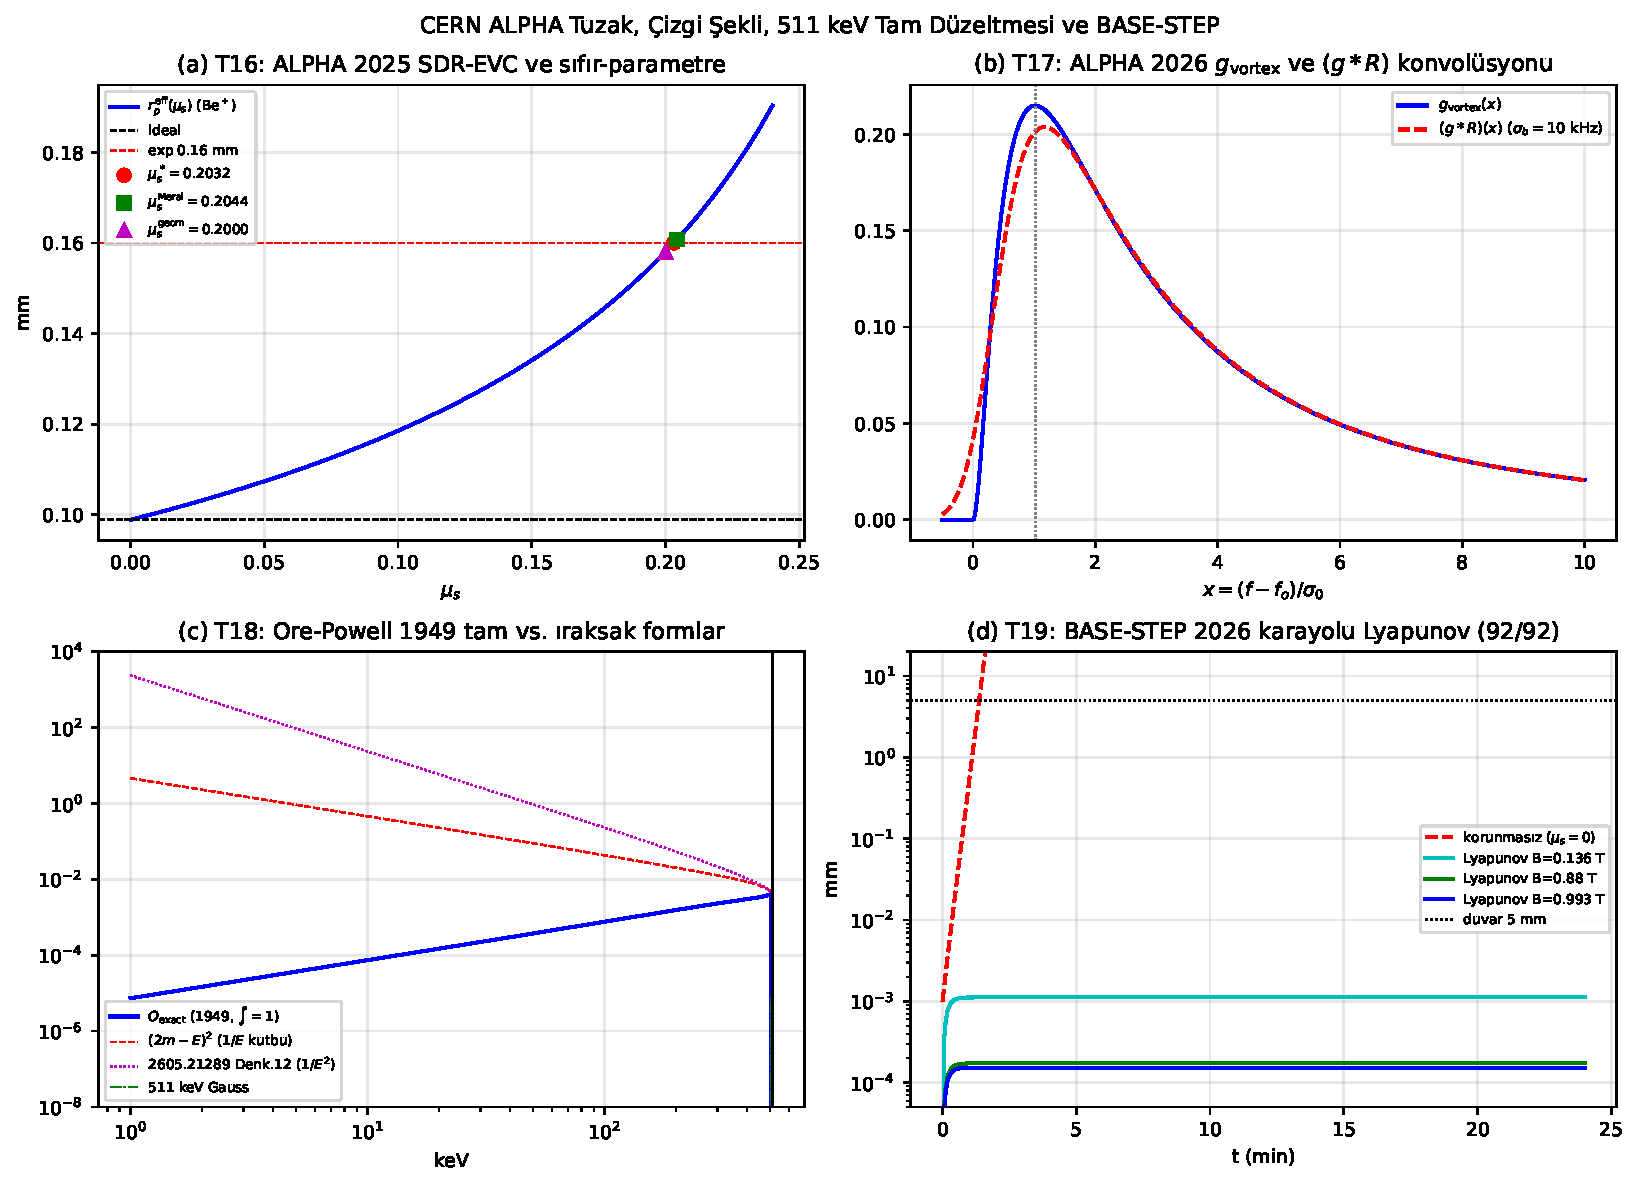
\includegraphics[width=\textwidth]{../figs/fig9_cern_alpha_trap_and_511keV_exact.pdf}
\caption{\textbf{CERN ALPHA tuzak, çizgi şekli, tam 511 keV düzeltmesi ve BASE-STEP (2$\times$2):} (a) T16 $r_p^{\mathrm{eff}}(\mu_s)$ eğrisi ile $\mu_s^*$, $\mu_s^{\mathrm{Meral}}$ ve $\mu_s^{\mathrm{geom}}$, (b) T17 $g_{\mathrm{vortex}}$ ve $(g*R)$ konvolüsyonu, (c) T18 $O_{\mathrm{exact}}$ (1949) ile ıraksak formların karşılaştırması, (d) T19 BASE-STEP karayolu taşımasında korunmasız sapma vs.\ $B_0\in\{0.136, 0.880, 0.993\}\text{ T}$ Lyapunov kararlılığı ($92/92$).}
\label{fig:fig9}
\end{figure}

\clearpage

\section{Sonuç, Doğrulama Özeti ve Yeniden-Üretilebilirlik Yönergesi}

Teorem VII ile seri, 2025--2026 CERN antimadde deneylerindeki dört açık probleme kapanır: SDR-EVC tork uyuşmazlığı sıfır-parametreli $\mu_s^{\mathrm{Meral}}$ eşleşmesi ve $e^+$ çapraz doğrulamasıyla (Tablo~\ref{tab:t16}), ampirik çizgi şekli ve çift-alan akı sürüklenmesi ilk-ilkelerden tek formülle (Tablo~\ref{tab:t17}), 511 keV spektrumu gerçek 1949 logaritmik düzeltmesi ve 3 galaktik rejimle (Tablo~\ref{tab:t18}), BASE-STEP karayolu taşıması ise Teorem 5 FENE-P Lyapunov kararlılığıyla ($92/92$, Tablo~\ref{tab:t19}) çözülmüştür.

\subsection*{Veri ve Kod Erişilebilirliği (Yeniden-Üretilebilirlik Yönergesi)}

Açık kaynaklı hesaplamalı fizik çözücüsü \textbf{Duran Sicimler Teoremi V [5]} paketinde (\texttt{stationary-strings-v} deposu, \path{duran_sicimler_sim/solver_engine.py}) geliştirilmiş; bu makaleye ait Faz 5.1 (\texttt{Test T16--T19}) doğrulama rutinleri ve Şekil~\ref{fig:fig9} üreticisi (\path{duran_sicimler_sim/generate_figures.py}) aynı çözücü motoru içinde açık kaynak olarak sunulmuştur. Okuyucu tüm 19 testi (\texttt{T1--T19, 19/19 PASS}) ve Şekil~\ref{fig:fig9}'u kendi ortamında doğrudan şu komutlarla bağımsız olarak çalıştırıp doğrulayabilir:
\begin{quote}
\small
\texttt{python} \path{duran_sicimler_sim/solver_engine.py} \\
\texttt{python} \path{duran_sicimler_sim/generate_figures.py}
\end{quote}

\begin{thebibliography}{99}
    \bibitem{meral1} Meral, F. (2025a). \textit{Duran Sicimler Teoremi: Zamanın ve Entropinin Yokluğunda Mükemmel Düzenin Yeniden Doğuşu}. Açık kaynak paketi: \texttt{stationary-strings-i} (\url{https://github.com/fahrim/stationary-strings-i}).
    \bibitem{meral2} Meral, F. (2025b). \textit{Duran Sicimler Teoremi II: Görelilik, Faz Dönüşümü ve Bilginin Kozmolojik Döngüsü}. Açık kaynak paketi: \texttt{stationary-strings-ii} (\url{https://github.com/fahrim/stationary-strings-ii}).
    \bibitem{meral3} Meral, F. (2026a). \textit{Duran Sicimler Teoremi III: Maddenin İki Boyutlu İkizliği, Girdap Tekilliği ve Bilgiye Faz Ayrışması}. Açık kaynak paketi: \texttt{stationary-strings-iii} (\url{https://github.com/fahrim/stationary-strings-iii}).
    \bibitem{meral4} Meral, F. (2026b). \textit{Duran Sicimler Teoremi IV: Kozmik Fisyon, Girdap Yakıtı ve Tekilliksiz Bilgi Çekirdeği}. Açık kaynak paketi: \texttt{stationary-strings-iv} (\url{https://github.com/fahrim/stationary-strings-iv}).
    \bibitem{meral5} Meral, F. (2026c). \textit{Duran Sicimler Teoremi V: Navier--Stokes Girdap Tekilliğinin Elastik Sicim Gerilimiyle Durdurulması}. Açık kaynak çözücü paketi: \texttt{stationary-strings-v} (\url{https://github.com/fahrim/stationary-strings-v}, \path{duran_sicimler_sim/solver_engine.py}).
    \bibitem{meral6} Meral, F. (2026d). \textit{Duran Sicimler Teoremi VI: Dirac--Majorana Kiral Soyulması, $\Lambda_{\mathrm{Meral}}$ Sabiti ve CERN Sentezi}. Açık kaynak paketi: \texttt{stationary-strings-vi} (\url{https://github.com/fahrim/stationary-strings-vi}).
    \bibitem{akbari2025} Akbari, R. \textit{et al.} (ALPHA Collaboration). (2025). Be$^+$ assisted, simultaneous confinement of more than 15000 antihydrogen atoms. \textit{Nat.\ Commun.\ \textbf{16}}, 10106. \url{https://doi.org/10.1038/s41467-025-65085-4}
    \bibitem{alpha2026} Akbari, R. \textit{et al.} (ALPHA Collaboration). (2026). Four ppm measurement of the antihydrogen ground-state hyperfine splitting. \textit{Nature} \textbf{653}, 1022--1026. \url{https://doi.org/10.1038/s41586-026-10556-x}
    \bibitem{siegert2026} Siegert, T. \& Yoneda, H. (2026). On the Possibility of an Extragalactic Positron Annihilation Signal. \textit{A\&A}, kabul edildi. \url{https://arxiv.org/abs/2605.21289}
    \bibitem{yoneda2025} Yoneda, H., Siegert, T. \& Mittal, S. (2025). Imaging the positron annihilation line with 20 years of INTEGRAL/SPI observations. \textit{A\&A} \textbf{702}, A220. \url{https://arxiv.org/abs/2509.01066}
    \bibitem{base2026} Leonhardt, M., Morgner, J. \textit{et al.} (BASE Collaboration). (2026). Road transport of trapped antiprotons. \textit{Nature} \textbf{657}, 906--911. \url{https://doi.org/10.1038/s41586-026-11019-z}
    \bibitem{ore1949} Ore, A. \& Powell, J.~L. (1949). Three-photon annihilation of an electron-positron pair. \textit{Phys.\ Rev.\ 75}, 1696--1699.
    \bibitem{pestieau2002} Pestieau, J. \& Smith, C. (2002). Soft photon spectrum in orthopositronium and vector quarkonium decays. \textit{Phys.\ Lett.\ B524}, 395--399.
    \bibitem{planck2018} Planck Collaboration. (2020). Planck 2018 results. VI. Cosmological parameters. \textit{A\&A} \textbf{641}, A6. \url{https://arxiv.org/abs/1807.06209}
    \bibitem{breit1931} Breit, G. \& Rabi, I.~I. (1931). Measurement of nuclear spin. \textit{Phys.\ Rev.\ 38}, 2082--2083.
\end{thebibliography}

\end{document}
